\documentclass[tikz,border=10pt]{standalone}
\usepackage[T1]{fontenc}
\usepackage{lmodern}
\usetikzlibrary{arrows.meta,backgrounds,calc}

\definecolor{ink}{HTML}{172033}
\definecolor{muted}{HTML}{59697F}
\definecolor{panel}{HTML}{F8FAFC}
\definecolor{panelborder}{HTML}{DCE5F0}
\definecolor{purple}{HTML}{7138E8}
\definecolor{purplefill}{HTML}{F0ECFF}
\definecolor{blue}{HTML}{2563EB}
\definecolor{bluefill}{HTML}{E1EDFF}
\definecolor{green}{HTML}{169B45}
\definecolor{greenfill}{HTML}{E1FBEA}
\definecolor{amber}{HTML}{D97706}
\definecolor{amberfill}{HTML}{FFF3C4}
\definecolor{red}{HTML}{C2410C}
\definecolor{redfill}{HTML}{FFF0E8}

\tikzset{
  card/.style={draw=purple,fill=white,line width=1.1pt,rounded corners=5pt},
  read/.style={-{Latex[length=2.6mm,width=2mm]},draw=blue,line width=1pt},
  read both/.style={{Latex[length=2.6mm,width=2mm]}-{Latex[length=2.6mm,width=2mm]},draw=blue,line width=1pt},
  shared/.style={-{Latex[length=2.6mm,width=2mm]},draw=amber,line width=1pt},
  label/.style={fill=panel,inner sep=2pt,font=\sffamily\bfseries\small},
}

\begin{document}
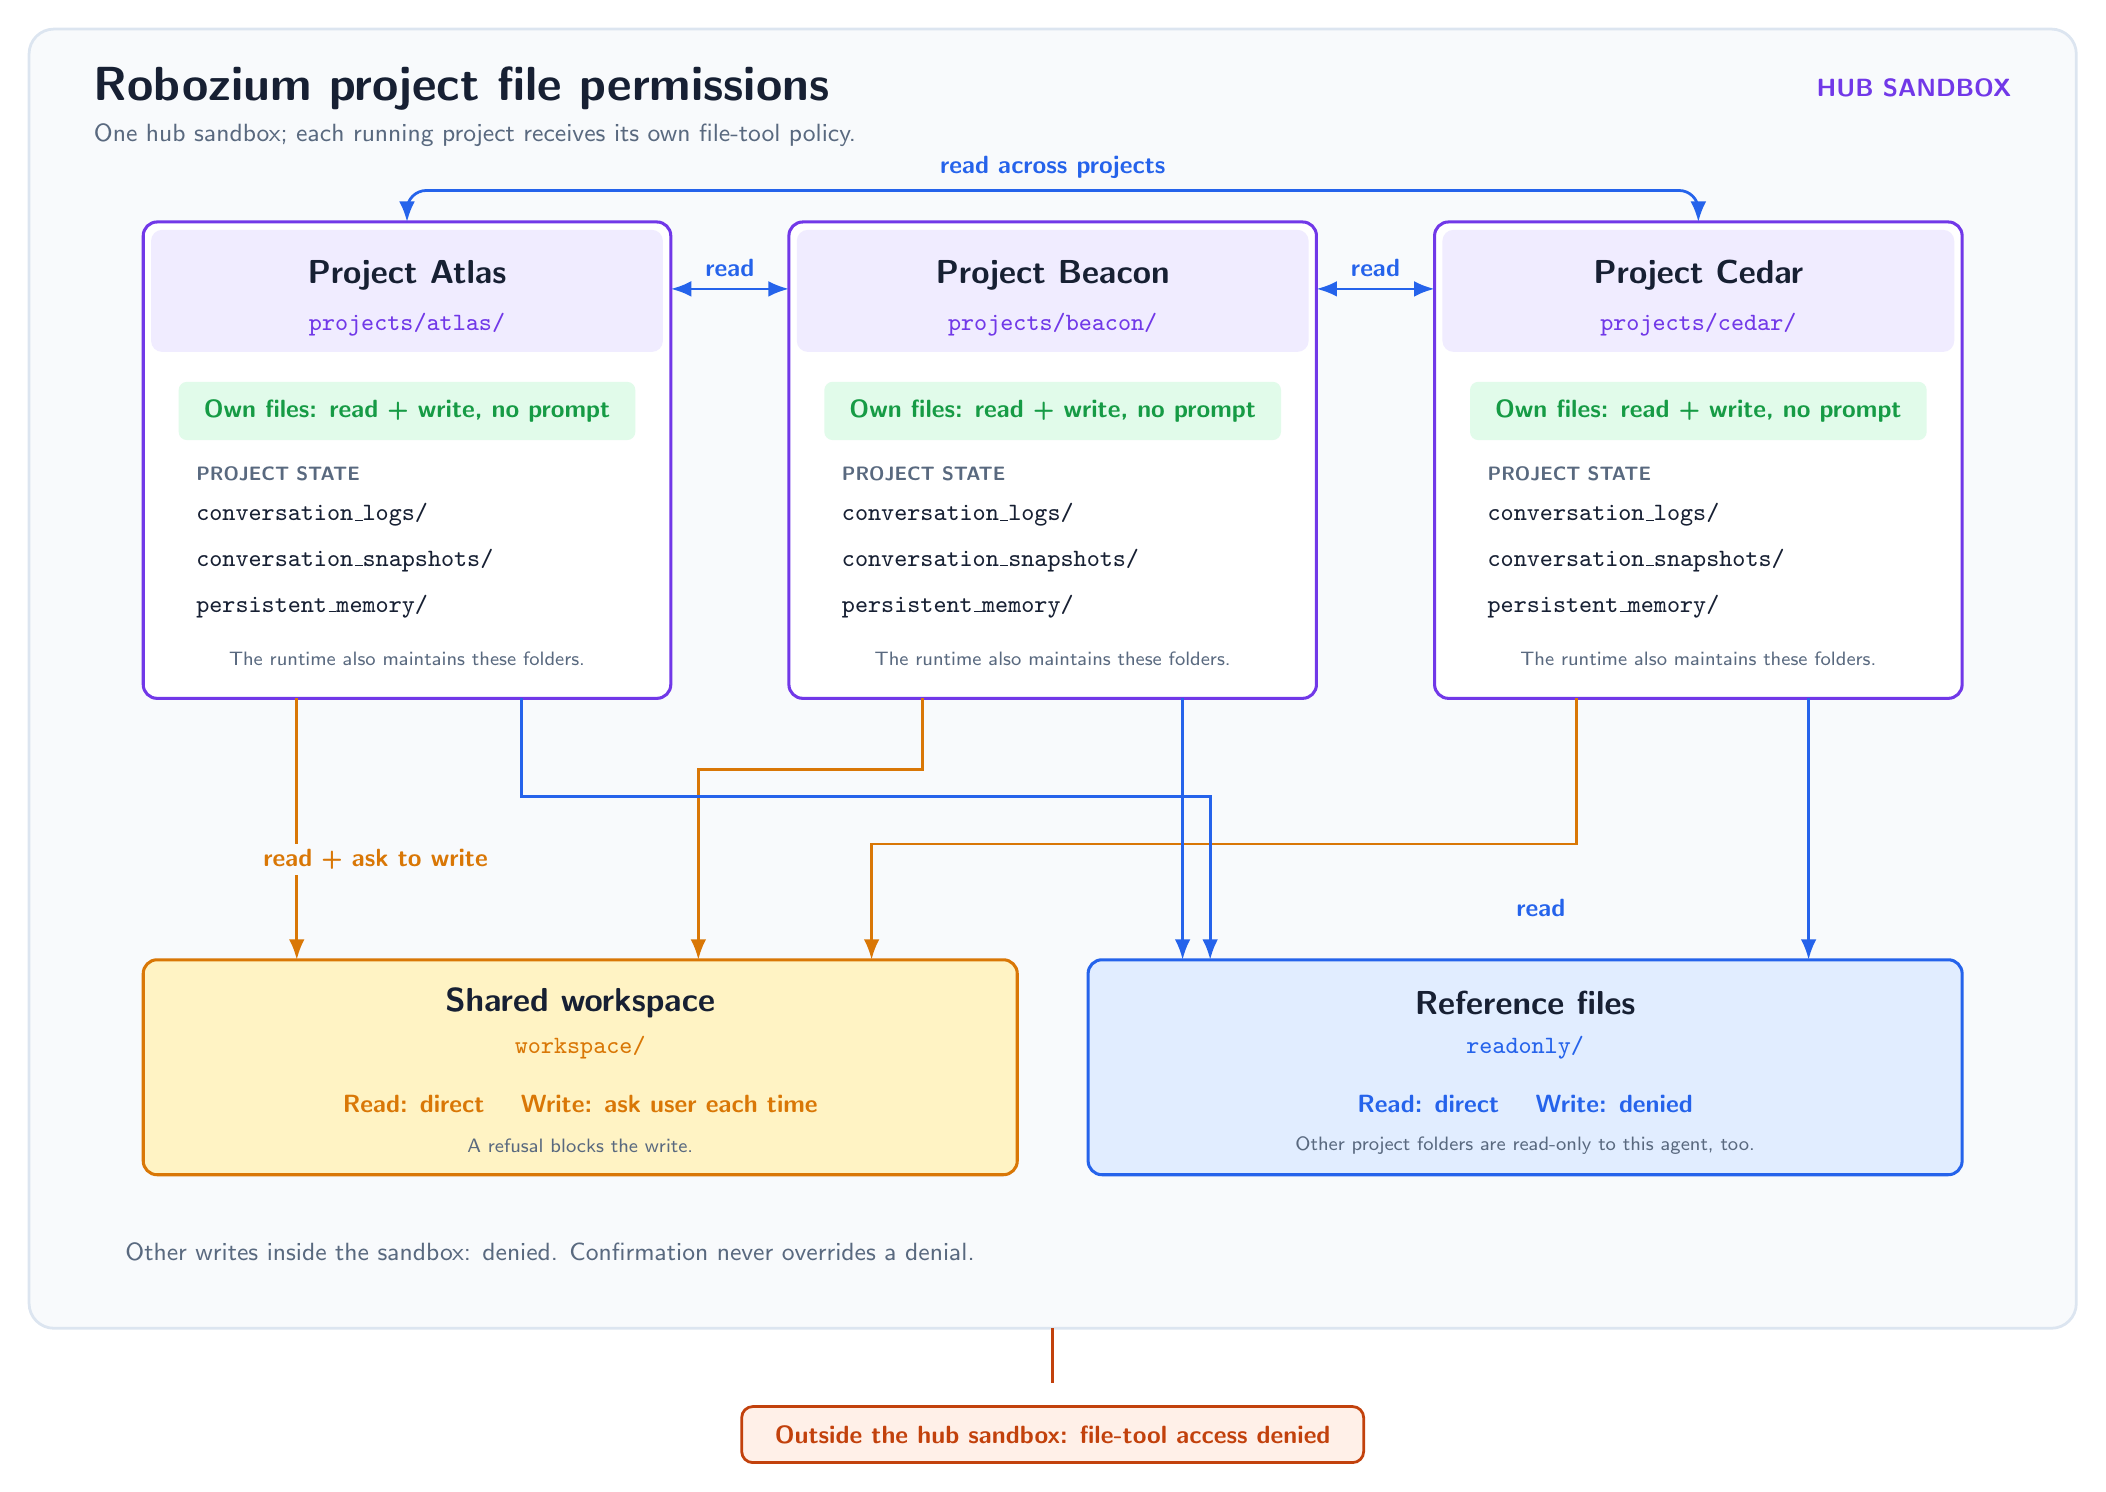
\begin{tikzpicture}[font=\sffamily]
  \begin{scope}[on background layer]
    \draw[draw=panelborder,fill=panel,line width=1pt,rounded corners=9pt]
      (0,3.1) rectangle (26,-13.4);
  \end{scope}

  \node[anchor=west,font=\sffamily\bfseries\LARGE,text=ink]
    at (0.7,2.35) {Robozium project file permissions};
  \node[anchor=west,font=\sffamily\small,text=muted]
    at (0.7,1.75) {One hub sandbox; each running project receives its own file-tool policy.};
  \node[anchor=east,font=\sffamily\bfseries\small,text=purple]
    at (25.3,2.35) {HUB SANDBOX};

  % Three illustrative projects. The green strip describes each project's own scope.
  \foreach \x/\slug/\title in {4.8/atlas/Atlas,13/beacon/Beacon,21.2/cedar/Cedar} {
    \draw[card] (\x-3.35,0.65) rectangle (\x+3.35,-5.4);
    \fill[purplefill,rounded corners=4pt] (\x-3.25,0.55) rectangle (\x+3.25,-1.0);
    \node[font=\sffamily\bfseries\large,text=ink] at (\x,-0.03) {Project \title};
    \node[font=\sffamily\small,text=purple] at (\x,-0.65) {\texttt{projects/\slug/}};
    \fill[greenfill,rounded corners=3pt] (\x-2.9,-1.38) rectangle (\x+2.9,-2.12);
    \node[font=\sffamily\bfseries\small,text=green] at (\x,-1.75)
      {Own files: read + write, no prompt};
    \node[anchor=west,font=\sffamily\bfseries\scriptsize,text=muted]
      at (\x-2.8,-2.55) {PROJECT STATE};
    \node[anchor=west,font=\sffamily\small,text=ink]
      at (\x-2.8,-3.07) {\texttt{conversation\_logs/}};
    \node[anchor=west,font=\sffamily\small,text=ink]
      at (\x-2.8,-3.65) {\texttt{conversation\_snapshots/}};
    \node[anchor=west,font=\sffamily\small,text=ink]
      at (\x-2.8,-4.23) {\texttt{persistent\_memory/}};
    \node[font=\sffamily\scriptsize,text=muted] at (\x,-4.9)
      {The runtime also maintains these folders.};
  }

  % Both directions mean each agent can read the other project's files.
  \draw[read both] (8.15,-0.20) -- node[label,text=blue,above=2pt] {read} (9.65,-0.20);
  \draw[read both] (16.35,-0.20) -- node[label,text=blue,above=2pt] {read} (17.85,-0.20);
  \draw[read both,rounded corners=7pt]
    (4.8,0.65) -- (4.8,1.05) --
    node[label,text=blue,above=2pt] {read across projects} (21.2,1.05) -- (21.2,0.65);

  % Shared destinations. Each arrow is drawn from one of the three projects.
  \draw[draw=amber,fill=amberfill,line width=1.1pt,rounded corners=5pt]
    (1.45,-8.72) rectangle (12.55,-11.45);
  \node[font=\sffamily\bfseries\large,text=ink] at (7,-9.27) {Shared workspace};
  \node[font=\sffamily\small,text=amber] at (7,-9.83) {\texttt{workspace/}};
  \node[font=\sffamily\bfseries\small,text=amber] at (7,-10.55)
    {Read: direct \quad Write: ask user each time};
  \node[font=\sffamily\scriptsize,text=muted] at (7,-11.08)
    {A refusal blocks the write.};

  \draw[draw=blue,fill=bluefill,line width=1.1pt,rounded corners=5pt]
    (13.45,-8.72) rectangle (24.55,-11.45);
  \node[font=\sffamily\bfseries\large,text=ink] at (19,-9.27) {Reference files};
  \node[font=\sffamily\small,text=blue] at (19,-9.83) {\texttt{readonly/}};
  \node[font=\sffamily\bfseries\small,text=blue] at (19,-10.55)
    {Read: direct \quad Write: denied};
  \node[font=\sffamily\scriptsize,text=muted] at (19,-11.08)
    {Other project folders are read-only to this agent, too.};

  % Upper and lower rails keep six access paths visible without obscuring cards.
  \draw[shared] (3.4,-5.4) -- (3.4,-8.72);
  \draw[shared] (11.35,-5.4) -- (11.35,-6.3) -- (8.5,-6.3) -- (8.5,-8.72);
  \draw[shared] (19.65,-5.4) -- (19.65,-7.25) -- (10.7,-7.25) -- (10.7,-8.72);
  \draw[read] (6.25,-5.4) -- (6.25,-6.65) -- (15,-6.65) -- (15,-8.72);
  \draw[read] (14.65,-5.4) -- (14.65,-8.72);
  \draw[read] (22.6,-5.4) -- (22.6,-8.72);
  \node[label,text=amber] at (4.4,-7.45) {read + ask to write};
  \node[label,text=blue] at (19.2,-8.06) {read};

  \node[anchor=west,font=\sffamily\small,text=muted] at (1.1,-12.43)
    {Other writes inside the sandbox: denied. Confirmation never overrides a denial.};

  % This is the boundary of the agent's file tools, not an OS-level container wall.
  \draw[red,line width=1.2pt] (13,-13.4) -- (13,-14.1);
  \node[draw=red,fill=redfill,line width=1pt,rounded corners=4pt,
        font=\sffamily\bfseries\small,text=red,inner xsep=12pt,inner ysep=7pt]
    at (13,-14.75) {Outside the hub sandbox: file-tool access denied};
\end{tikzpicture}
\end{document}
